%kelompok 1 Sistem Operasi (firmata, komunikasi arduino)
%Kelas D4 TI 1B
%Adam Noer Hidayatullah 1174097
%Ichsan Hizman Hardy 1174034
%Teddy
%Nisrina Aulia
%Irvan Rizkiansyah 1174043

\section{Firmata, komunikasi arduino}
	Sebenarnya arduino sudah menyediakan IDE sendiri untuk melakukan sebuah project yang menggunakan arduino sehingga lebih mudah dan kinerja yang bagus, akan tetapi tidak ada yang melarang untuk menggunakan development tools yang lainnya seperti :
	\begin{itemize}
		\item Dataino
		\item Processing 2
		\item Firmata
		\item Arduino VB Lab
	\end{itemize}
	Namun kali ini yang akan dibahas adalah Firmata.
	
	\subsection{Firmata}
	Firmata adalah protocol yang ditulis pada Arduino untuk memudahkan komunikasi serial Arduino dengan sesama software di komputer. Firmata pun support berbagai macam sistem operasi tidak hanya pada windows saja, melainkan seperti linux, MacOSX pun support firmata. Dibawah ini adalah contoh test Firmata pada MacOSX.
	
	\begin{figure} [ht]
		\centerline{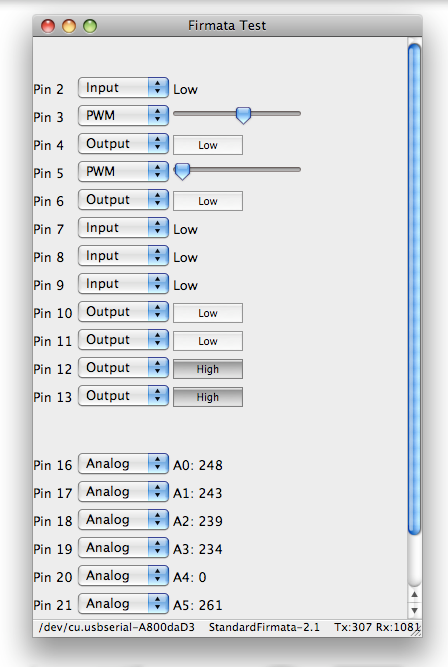
\includegraphics[width=1\textwidth]{figures/firmatates.png}}
		\caption{Gambar Contoh Test Firmata MacOSX}
		\label{firmatates}
	\end{figure}
	
	\ref{firmatates}
	
	\subsubsection{Methods}
		\begin{verbatim}
			begin(); //start the library
			begin(long); //start the library and override the default baud rate
			begin(Stream s); 
			printVersion(); 
			blinkVersion(): 
			printFirmwareVersion(); 
			setFirmwareVersion(byte major, byte minor); 
			setFirmwareNameAndVersion(const char *name, byte major, byte minor); 
		\end{verbatim}
		
		\begin{itemize}
			\item Sending Messages
				\begin{verbatim}
					sendAnalog(byte pin, int value); //send an analog message
					sendDigitalPort(byte portNumber, int portData); //send an 8-bit port in a single digital message
					sendString(const char* string); 
					sendString(byte command, byte bytec, byte bytev); 
					sendSysex(byte command, byte bytec, byte bytev); 
					write(byte c); 
				\end{verbatim}
			\item Receiving Messages
				\begin{verbatim}
					available(); 
					processInput(); 
					attach(byte command, callbackFunction myFunction); 
					detach(byte command); 
				\end{verbatim}
		\end{itemize}
	
	\subsubsection{Utility Methods}
		\begin{verbatim}
			sendValueAsTwo7bitBytes(int value); 
			startSysex(void); 
			endSysex(void); 
		\end{verbatim}
	
	\subsection{LabVIEW}
	LabVIEW memiliki fungsi yang sama seperti firmata tetapi lebih mudah, mudah dalam arti pemrograman tidak lagi dilakukan di kedua sisi,
	tetapi hanya di satu sisi, yaitu di software komputer saja.
	
	\subsection{Fungsi Firmata}
	contoh fungsi firmata adalah dapat mengontrol Arduino menggunakan software seperti LabVIEW, MATLAB, dll, tanpa harus memprogram khusus di Arduino.
	
	\subsection{MATLAB}
	MATLAB adalah salah satu software yang sepenuhnya mengambil kontrol pda arduino fungsinya akan menghemat waktu dalam mengintegrasi MATLAB arduino.
	
	\subsection{Interaksi Arduino dan LabVIEW}
	Interaksi antara Arduino dengan LabVIEW dikarenakan masing-masing mempunyai kelebihan dan kekurangan masing-masing, apabila keduanya digabungkan akan saling menambahkan, namun akan sebaliknya kekurangan yaitu kekurangannya keduanya akan saling mentiadakan.
	
	\subsection{Menginstall Firmata}
	Menginstal Firmata di LabVIEW disebut dengan LabVIEW Interface For Arduino (LVIFA). fungsingnya yaitu dapat membaca sinyal analog potensio,
	pembaca sensor seperti thermistor,LDR, joystick.
	
	Dirangkum dari jurnal \cite{steiner2009firmata}
	Dirangkum dari jurnal \cite{majocchi2012arduino}